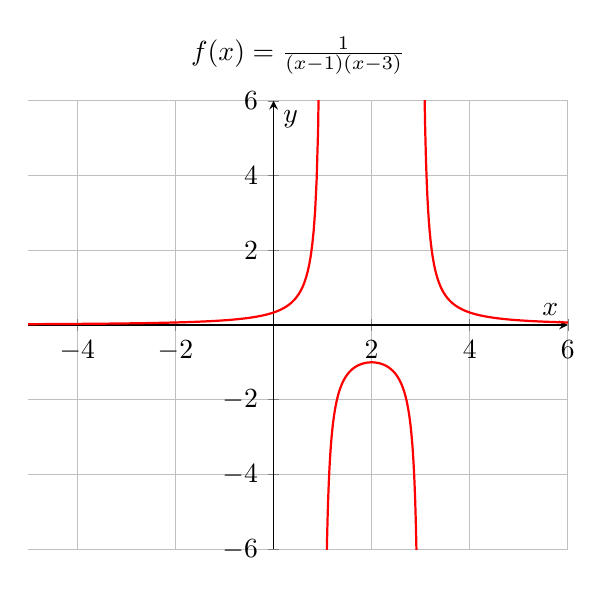
\begin{tikzpicture}
    \begin{axis}[
      title={$f(x) = \frac{1}{(x-1)(x-3)}$},
        axis lines = middle,
        grid = major,
        xmin = -5, xmax = 6,   % Ajusta la ventana en x
        ymin = -6, ymax = 6,   % Ajusta la ventana en y
        xlabel={$x$},
        ylabel={$y$},
        unbounded coords=jump, % Salta en lugar de trazar líneas infinitas
        samples=200            % Más puntos para una curva suave
    ]
    % Graficar f(x) en tres intervalos separados:
    %  1) Desde x=-5 hasta justo antes de x=1
    \addplot[domain=-5:0.999, thick, red]
      {1/((x-1)*(x-3))};

    %  2) Desde un poco después de x=1 hasta antes de x=3
    \addplot[domain=1.001:2.999, thick, red]
      {1/((x-1)*(x-3))};

    %  3) Desde un poco después de x=3 hasta x=6
    \addplot[domain=3.001:6, thick, red]
      {1/((x-1)*(x-3))};

    \end{axis}
\end{tikzpicture}